\section{PWA-alternatieven}

In deze sectie zal er onderzoek gedaan worden naar technologieën waarbij er een applicatie ontwikkeld kan worden die op meerdere platformen kan werken waarbij er ook maar 1 codebase is. Er zal gekeken worden wat de voor- en nadelen zijn van deze technologieën. 

Het doel van cross platform ontwikkeling is dat het gemakkelijker en sneller moet zijn om een applicatie te creëren en te onderhouden voor meerdere platformen.

Het ontwikkelen van een applicatie aan de hand van een cross platform development benadering zal minder tijd in beslag nemen, aangezien er minder code moet geschreven worden, dan het ontwikkelen van native toepassingen voor meerdere platformen. 

Een ander voordeel van deze technologie is dat het gemakkelijker is om consistent te zijn met een applicatie over meerdere platformen. Als een applicatie op de traditionele manier wordt ontwikkeld, is er vaak een team voor elk platform. Deze teams maken dezelfde applicatie, maar voor een ander platform. Dit heeft als gevolg dat beide applicaties niet 100\% gelijk zullen zijn. Dit kan de gebruiker verwarren.


\subsection{Cross platform hybrid development}

	Hybride mobiele applicaties zijn applicaties waarbij de userinterface weergeven wordt in een minimale versie van een webbrowser.
		
	Dit type applicatie kan gebouwd worden met de technologieën die beschikbaar zijn voor het web.
	
	Bij het creëren van een hybride applicatie wordt er een minimale browser aangemaakt in het package van de applicatie. De applicatie wordt vervolgens in deze minimale browser gebouwd. Deze combinatie van bestanden kan vervolgens geüpload worden naar platformen zoals de Google Play store of de App Store van Apple.
	\autocite{Huynh2017}
	
	
	\subsubsection{Voordelen}
		Het grote voordeel van hybride applicaties is dat de overstap van web development naar het ontwikkelen van hybride applicaties heel klein is. De technologieën die gebruikt worden bij web-ontwikkeling kunnen overgenomen worden om mobiele applicaties te ontwikkelen. Er moeten dus geen nieuwe frameworks of technologieën geleerd worden.
		
		Dit betekent ook dat de vele libraries en packages die beschikbaar zijn voor het web ook gebruikt kunnen worden voor app-ontwikkeling.
		
		Hybride applicaties hebben in tegenstelling tot webapplicaties en PWA’s wel toegang tot alles wat een besturingssysteem beschikbaar stelt voor applicaties. Een hybride applicatie heeft bijvoorbeeld wel volledige toegang tot het sms-verkeer van een toestel 
		\autocite{Ionic2020}
	
	\subsubsection{Nadelen}
		De userinterface die gemaakt wordt aan de hand van een hybride applicatie is op elk toestel dezelfde. Dit zorgt ervoor dat de app niet intuïtief aanvoelt. Een native Androidapplicatie heeft bijvoorbeeld een ander navigatiesysteem dan een IOS-applicatie. Bij het maken van een hybride oplossing zal deze navigatie op beide platformen dezelfde zijn.
		
		De prestaties van een website die in een webview werkt zijn minder goed dan bij een native applicatie.
		\autocite{Asp2017}	

		
	\subsubsection{Apache cordova}
		Apache Cordova is een technologie die een website ontsluit in een webview. Deze webview kan gezien worden als een basisversie van een gewone mobiele browser zonder interface-elementen zoals een url-veld of een statusbar. Er bestaan ook veel plugins die het gemakkelijk maken om de functies van het besturingssysteem te gebruiken. Voorbeelden hiervan zijn het gebruik van de camera of de flashlight.
		
		
	\subsubsection{Ionic}
		Ionic is een framework voor het bouwen van hybride applicaties. Het maakt gebruik van de webview die cordova aanbiedt.
		
		De functionaliteiten die Ionic aanbiedt kunnen gebruikt worden met de populaire frontend frameworks: Angular, React en Vue.
		
		Ionic framework heeft ook een ruime bibliotheek aan plug-ins die ervoor zorgen dat een applicatie gebruik kan maken van de functies die een besturingssysteem heeft.
		
		Een applicatie die ontwikkeld is in Ionic, kan gepubliceerd worden in de Apple app-store, de Google Play-store en ook als PWA. Verschillende plugins die gebruikt kunnen worden voor de native applicaties kunnen ook gebruikt worden voor PWA’s. Ionic is dus heel geschikt voor cross platform development. 
		\autocite{Ionic2020a}
		
		De ontwikkelervaring van een Ionic applicatie is ook aangenaam omdat Ionic ‘live reloading’ ondersteunt. Dit wil zeggen dat de applicatie niet opnieuw “gebuild” moet worden om de aanpassingen te zien. 
		\autocite{Lucas2020}
		
		Het Ionic framework zal er ook voor zorgen dat de applicatie meer native aanvoelt door de UI-elementen die het aanbiedt. Als een applicatie “gebuild” wordt zal Ionic ervoor zorgen dat de juiste UI-componenten voor elk toestel gebruikt worden. Zo zal een Androidapplicatie het material design volgen en een IOS-applicatie het human design. 
		
		Een Ionic applicatie zal meer middelen vragen van een toestel. Als prestaties een belangrijke factor zijn bij de applicatie die gebouwd moet worden, is deze hybride benadering dus niet ideaal.
		
		Een Ionic applicatie is zowel intensief voor de CPU als voor de batterij. Wat wel opvallend is, is dat de grootte van een applicatie kleiner is dan bij cross platform native development. 
		\autocite{Asp2017}	


	\subsubsection{Electron}
		Electron is een framework dat gebruikt kan worden om desktopapplicaties te bouwen, gebruik makende van web technologieën.  De code kan gecompileerd worden naar een native programma voor Linux, Mac en Windows.
		
		Een applicatie die geschreven is met Electron heeft, in tegenstelling tot een website, wel de rechten om bestanden op het toestel aan te passen of aan te maken.
		
		Electron voorziet ook API’s om gebruik te maken van geavanceerde functionaliteiten zoals het bestandssysteem en bluetooth.
		
		Een groot voordeel van ontwikkelen met Electron is dat Chromium gebruikt wordt als webview. Dit zorgt ervoor dat een applicatie zich op elk besturingssysteem gelijk zal gedragen. Dit zorgt er ook voor dat de ontwikkelaar toegang heeft tot de ‘Developer Tools’ die normaal gebruikt worden bij het ontwikkelen van een webapplicatie. 
		
		Een van de grote nadelen van Electron is dat het startproject al heel groot is. De Chromium webview heeft alleen al meer dan 20 miljoen lijnen code. Dit zorgt ervoor dat Electron enkel interessant wordt voor heel grote projecten waarbij dit gerechtvaardigd kan worden.
		De code is ook niet geëncrypteerd. Dit wil zeggen dat een gebruiker die een programma downloadt aan de broncode kan van dit programma. Als de code van een applicatie niet beschikbaar mag zijn, kan Electron niet gebruikt worden.
		
		Voorbeelden van software die ontwikkeld zijn met Electron zijn:
		\begin{itemize}
			\item	Slack
			\item	Visual studio code
			\item	Discord
		\end{itemize}

		
		

\subsection{Cross platform native development}
Het grote verschil met hybrid applications is dat bij cross platform native development de code gecompileerd wordt naar native componenten. Er wordt dus geen webview gebruikt.
\autocite{Ghinea2018}
\autocite{DeConinck2019}

	\subsubsection{Voordelen}
		De meeste cross platform development frameworks hebben een functie ‘hot reload’. Dit wil zeggen dat de app tijdens het ontwikkelen op een emulator kan uitgevoerd worden. Elke keer een verandering aangebracht wordt, zal deze app direct updaten. Dit vereenvoudigt het ontwikkelproces. 
		
		Bij cross platform development wordt de code omgevormd tot native componenten. Dit zorgt ervoor dat een applicatie een meer ‘native feeling’ zal hebben dan bij hybrid applications. Een knop die gecompileerd wordt naar Android zal er anders uitzien dan een knop die gecompileerd wordt naar IOS.
		\autocite{Asp2017}
	
	\subsubsection{Nadelen}
		De prestaties zijn dan wel beter dan bij een hybrid applicatie, maar voor applicaties die veeleisend zijn op vlak van CPU en geheugen zijn cross platform development frameworks niet de beste oplossing. Hier wordt beter een native oplossing gebruikt waarbij er toch nog twee of meer codebases zijn.
		\autocite{Asp2017}
		
		
	\subsubsection{Xamarin}
		Xamarin is een platform die gebruikt kan worden om applicaties voor Android, IOS, Windows en Mac OS te maken.  Xamarin is ontwikkeld en wordt onderhouden door Microsoft. De taal en technologie die bij dit platform gebruikt wordt is C\#. Naar schatting kan 90\% van de code in C\# geschreven worden. De resterende 10\% van de code moet nog steeds geschreven worden in de taal van het platform zoals Java voor Android, Swift voor IOS. De code die niet met C\# geschreven is, is de code die de userinterface maakt.
		\autocite{Altexsoft2019} \autocite{Warcholinski2020}
		
		De IDE Visual studio voorziet veel tools die het ontwikkelen van Xamarin applicaties makkelijker maakt.
		\autocite{VisualStudio2020}
		
		
		Bij ontwikkeling met Xamarin kan er ook gebruik gemaakt worden van Xamarin forms. Dit is een library die native componenten voorziet voor verschillende besturingssystemen. Zo zal elk component er verschillend uitzien op verschillende platformen, dit om aan het verwachtingspatroon van de gebruiker te voldoen.
		\autocite{Microsoft2019}
	
		Xamarin is het framework die de cross-platform trend heeft gestart. Het platform werd begin 2013 uitgebracht. Doordat het al enkele jaren bestaat, zijn er al veel vragen gepost op fora, waardoor de kans groot is dat, als een ontwikkelaar een probleem heeft, dit gedocumenteerd staat op een forum.
		
		Dit is ook terug te zien in het aantal zoekopdrachten op Stackoverflow. Bij de categorie ‘frameworks’ staat Xamarin op de 10e plaats. Enkel React native en Cordova staan hoger op deze lijst.
		\autocite{StackOverflow2020}
		
	\subsubsection{React native}
		React native\autocite{Reactnative2020}) is een framework gebaseerd op React.js. Beide frameworks zijn ontwikkeld en worden onderhouden door Facebook en worden geschreven in JavaScript. Bij React native moeten bepaalde specifieke onderdelen nog geschreven worden in de native codeertaal. 
		
		Het voordeel van React.js en React native is dat er een ‘learn once, write anywhere’ benadering is. React.js en React native zijn heel gelijkaardig, dit zorgt er dus voor dat een ontwikkelaar maar 1 technologie moet leren en dan voor zowel web als mobiel kan ontwikkelen.
		
		React native maakt gebruik van een concept genaamd ‘bridges’. Dit is de vertaling die gemaakt wordt van JavaScript naar native. React native voorziet deze ‘bridges’ voor de veel voorkomende items zoals een button, een text field, een calendar. Als er meer specifieke en minder courante functies gebruikt worden, moeten deze bridges zelf geschreven worden. Deze bridges moeten geschreven worden in de taal van het platform. 
		\autocite{Bartosz2019}
		
		React native was het eerste cross-platform framework dat grote successen kende. Hierdoor is er al een grote online community waar je terecht kan bij eventuele problemen. Dit is ook terug te zien in het aantal zoekopdrachten op stackoverflow. Bij de categorie ‘frameworks’ staat React native op de 6e plaats. Dit is het hoogst genoteerde framework dat mobiele applicaties produceert.
		\autocite{StackOverflow2020}
		
		
		\paragraph{Expo}
			Expo is een verzameling van tools die aan React native toegevoegd worden. Het levert bijvoorbeeld een command line interface. Expo zorgt ervoor dat een volledige applicatie geschreven kan worden met enkel gebruik te maken van JavaScript. Hierdoor is de combinatie van React native en Expo populair bij webdevelopers.
			
			Expo heeft het doel om de ontwikkeltijd van een applicatie zo laag mogelijk te houden. Een voorbeeld hiervan is dat de ontwikkelaar een applicatie kan downloaden op zijn toestel waarin de applicatie die ontwikkeld wordt, getest kan worden. Ook zijn functionaliteiten zoals push-notifications voorzien door Expo.
			
			Expo heeft verschillende API’s om toegang te krijgen tot de verschillende functies van een toestel. De meeste applicaties kunnen gebouwd worden door gebruik te maken van deze API’s. 
			
			Het gebruik van Expo kan echter ook limiterend zijn voor een applicatie. Als ontwikkelaar ben je volledig afhankelijk van deze API’s. Er kan enkel JavaScript geschreven worden en dus geen native code zoals dit bij een traditioneel React native project wel mogelijk is.
			Een React native project dat gebruik maakt van Expo heeft nu ook webondersteuning. Dit houdt in dat een applicatie geschreven wordt in JavaScript en kan geëxporteerd worden naar een IOS app, Android app en een PWA.
			
			Deze functionaliteit is nog in de Beta fase en er wordt aangeraden dit nog niet te gebruiken in productie.
			\autocite{Expo2020}


	\subsubsection{Flutter}
		Flutter \autocite{Flutter2020} is een relatief nieuw framework voor het ontwikkelen van mobiele applicaties. De programmeertaal die gebruikt wordt bij Flutter is Dart. Zowel Flutter als Dart zijn gecreëerd en worden onderhouden door Google. 
		
		Net zoals React native is het nu ook mogelijk om een PWA te maken aan de hand van Flutter. Ook bij Flutter is het nog niet aangeraden om dit al effectief te gebruiken omdat PWA-ondersteuning nog in de beta fase is. 
		
		Flutter zorgt er ook voor dat een project 100\% in Dart geschreven kan worden. Er is dus geen nood om native talen te leren. 
		
		Een nadeel is dat Flutter een heel nieuw framework is en dat er online minder hulp te vinden zal zijn voor de ontwikkelaar dan bij React native. Dit is ook terug te zien in het aantal zoekopdrachten op stackoverflow. Bij de categorie ‘frameworks’ staat Flutter slechts op de 12e plaats. Dit is slechts het 4e framework voor app development.
		\autocite{StackOverflow2020}
		
\subsection{Conclusie}

Er kan geen duidelijk antwoord geformuleerd worden over welke technologie er “de beste” is. Dit zal steeds afhangen van het doel van de applicatie en de achtergrond die de ontwikkelaar heeft.


In een eerste fase moet er  bekeken worden als het technisch mogelijk is om de applicatie te ontwikkelen als PWA. Als de applicatie functionaliteiten bevat die enkel beschikbaar baar zijn voor native applicaties, is een PWA geen optie meer.

Als er beslist wordt dat een PWA geen optie is, zijn er nog steeds twee keuzes: een hybride applicatie of een native applicatie. Bij deze beslissing is het belangrijk om te kijken naar wat het doel en het doelpubliek is van de applicatie. Als de meeste gebruikers verwacht worden op het web, is een hybride applicatie een goede oplossing. De ondersteuning van hybride applicaties is heel goed voor websites. Dit is iets was nog niet op punt staat bij native cross platform benaderingen. Ionic is het meest gebruiksvriendelijk platform om hybride applicaties te ontwikkelen.

Als de meeste gebruikers verwacht worden op native code, is cross platform native ontwikkeling de beste optie. De applicatie wordt omgezet naar native componenten en dit zorgt voor een meer ‘native gevoel’. De gebruikerservaring zal beter zijn.

Als de keuze gemaakt is om native cross platform development toe te passen, zijn er nog steeds verschillende opties. Hier zal de achtergrond van de ontwikkelaar een grote rol spelen in welke technologie de optimale zal zijn. Ontwikkelaars met een web en JavaScript achtergrond kunnen gemakkelijk de overstap maken naar React native en Expo. 

Voor ontwikkelaars met een C\# achtergrond is een applicatie in Xamarin een vanzelfsprekende keuze. 

Flutter is geschreven in een nieuwe taal, Dart,  waar niet veel ontwikkelaars een achtergrond in hebben. Maar Dart leunt dicht bij Java, dus voor ontwikkelaars die hier ervaring in hebben, is Flutter de logische keuze.

Als er in geen van deze talen of technologiën een achtergrond is, is Flutter een goeie keuze.
\autocite{Leler2017}
\autocite{Wenhao2018}

Flutter belooft een snellere ontwikkeltijd en is heel performant. Het is ook een groot voordeel dat er geen native code geschreven moet worden.
Deze belofte wordt ook bevestigd door het onderzoek dat Jakub Fagietto voerde.
\autocite{Fagietto2019}


\subsection{Concluderende flowchart}
\begin{figure}[]
	\centering
	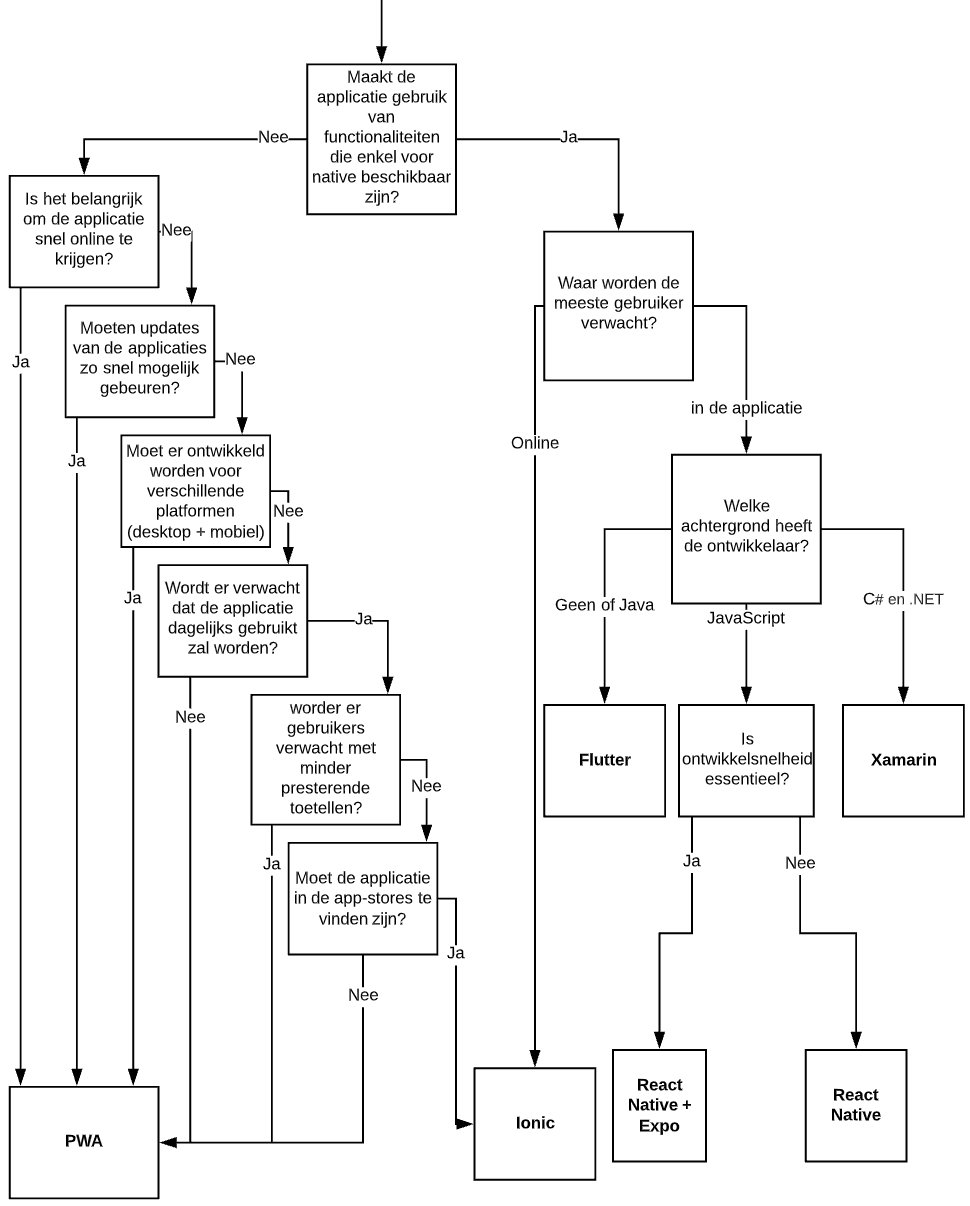
\includegraphics{./img/flowchart.png}
	\caption{flowchart: technologieën met één codebase die op meerdere platformen gebruikt kunnen worden}
\end{figure}

\clearpage


